\documentclass[my_thesis.tex]{subfiles}

\begin{document}
\cleardoublepage
\chapter{Introduction}
\markboth{Introduction}{Introduction}
\addcontentsline{toc}{chapter}{Introduction}
 

Our civilization needs a new source of energy, and it needs to be nuclear fusion energy. In this introduction, we motivate this statement by looking at why energy is a crucial ingredient of human development. We discuss the available energy sources today, their advantages and disadvantages, and introduce the nuclear fusion reaction. We then focus on the stellarator, which is a nuclear fusion power plant concept which uses 3-dimensional magnetic fields to confine a thermonuclear plasma, in which fusion reactions take place.

\section{Energy consumption and quality of life}

The Human Development Index (HDI)  \citep{undp1990} is a composite statistic used to rank countries by their level of human development. It was developed by the United Nations Development Programme (UNDP) as an alternative to traditional measures of development, such as gross domestic product (GDP), which do not take into account other important dimensions of well-being such as health, education, and living standards. The HDI is a measure of the average achievements of a country in these three dimensions, calculated using life expectancy at birth, mean years of schooling, and gross national income per capita. On Figure \ref{fig.hdi}, we show the HDI as a function of the average energy consumption per inhabitant, for a wide range of different countries. One striking observation is that the HDI grows with the energy consumption per inhabitant --- in other words, the more energy is available, the higher the quality of life is.

\begin{figure}
    \centering
    \subfloat{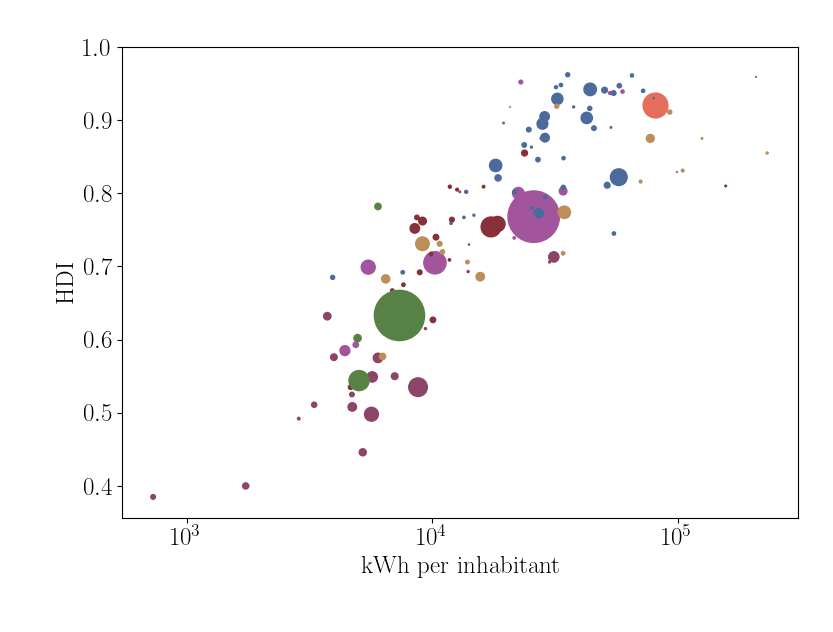
\includegraphics[width=\linewidth]{images/HDI_fct_kWh.png}}\\
    \centering
    \subfloat{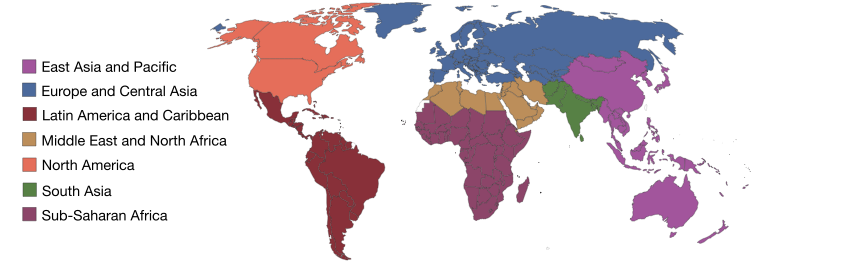
\includegraphics[width=\linewidth]{images/WorldMap.png}}
    \caption{Top: HDI as a function of the average energy consumption per country's inhabitant. Size of dots are proportionals to the total population of the country. Colors indicate the region the country belongs to, according to the World Bank classification. Bottom: regions defined by the World Bank classification. The HDI data were obtained from the UNDP website (\url{hdr.undp.org}, consulted the 26.12.2022), while the energy consumption in each country and its number of inhabitant were obtained from the World Bank website (data.worldbank.org, consulted the 26.12.2022). The data dates from 2014; at the time of writing this thesis, there were no extensive dataset that postdates 2014.}
    \label{fig.hdi}
\end{figure}

Indeed, countries with the higher HDI are often the most developed. Energy is a critical factor in human development because it plays a vital role in supporting economic growth and improving people's quality of life. Access to energy allows people to participate in economic activities, access education and healthcare, and improve their living standards. For example, access to electricity can enable people to use appliances, lighting, and other modern technologies that can improve their living conditions and increase their productivity. It can also facilitate the provision of basic services such as healthcare and education. Similarly, the availability of energy can support economic development by enabling the production of goods and services, improving transportation, communication, and other essential activities.

While the Human Development Index (HDI) is a widely used measure of human development, it is important to recognize its limitations \citep{mcgillivrayMeasuringDevelopmentUNDP1993a,bagolinHumanDevelopmentIndex2008,dervisMeasuringHumanProgress2011}. The HDI is based on three indicators, but it does not capture many other important aspects of human well-being. There have been proposals for alternative measures of human development that address some of these limitations (see for example the work by \citet{biggeriMoreSustainableHuman2018}, and references therein), but none of these have gained the same level of attention as the HDI. It is also worth considering that there may be cultures where the concept of happiness and success does not align with having a high HDI. These philosophical debates about the limitations of the HDI have been ongoing for many years and are beyond the scope of this thesis. However, it is worth noting that one potential solution to the energy problems facing the world today may be to change our consumption patterns and potentially accept a lower HDI. This thesis instead explores the opposite possibility of finding a new source of energy as a way to sustain our current way of life.

\section{The need for a new source of energy}

There are three main categories of energy sources: renewable energies, fossil fuels, and nuclear energy. Each energy source have its own advantages and disadvantages, discussed briefly below. A more extensive discussion can be found in numerous books; for instance, see \citet{parisiFutureFusionEnergy2018}.

\subsubsection{Renewable energies}
Renewable energies, such as solar, wind, hydropower, biomass, and geothermal, are not depleted once consumed and have been in use for centuries. Some examples of renewable energy include windmills powered by wind, or the use of wood as an energy source for cooking and heating households. In the recent years, these energy sources have gained increasing public and private traction as a mean to transition from a fossil energy based economy to a renewable economy, and fight the anthropological generated climate change \citep{allanIPCC2021Summary}. Indeed, one of the main advantage of renewable energy sources is that they do not produce greenhouse gases, which are the main drive to climate change. In addition, renewable energies are widely available, even in the most remote areas of the globe. In consequence, the energy production can often be located close to the energy consumer, thereby reducing the need for large infrastructures to transport energy. Being widely available also contribute to the geopolitical stability, as there are less dependencies between countries.

However, renewable energies also have disadvantages. Their energy density is relatively low, and large portion of land have to be used for power plants. For example, hydropower uses about $14\text{m}^2$ per MWh, and solar panels $13\text{m}^2$ per MWh (if installed on the ground) \citep{ritchieHowDoesLand2022}. This means that large areas have to be used for energy production, and large structures have to be built. Another challenge of renewable energy sources is their intermittent nature - solar panels only produce energy during the day and wind turbines only when there is wind. Energy storage, such as through water pumping, hydrogen production, or large batteries, can help mitigate this issue, but it comes with energy losses and can only be scaled up to meet global demand with massive infrastructural changes. As a result, renewable energies alone probably cannot provide a consistent base-load power supply to the grid. In 2021, about 12 \% of the total consumed energy was produced by renewable sources (see Figure \ref{fig.energy consumption}).

\begin{figure}
    \centering
    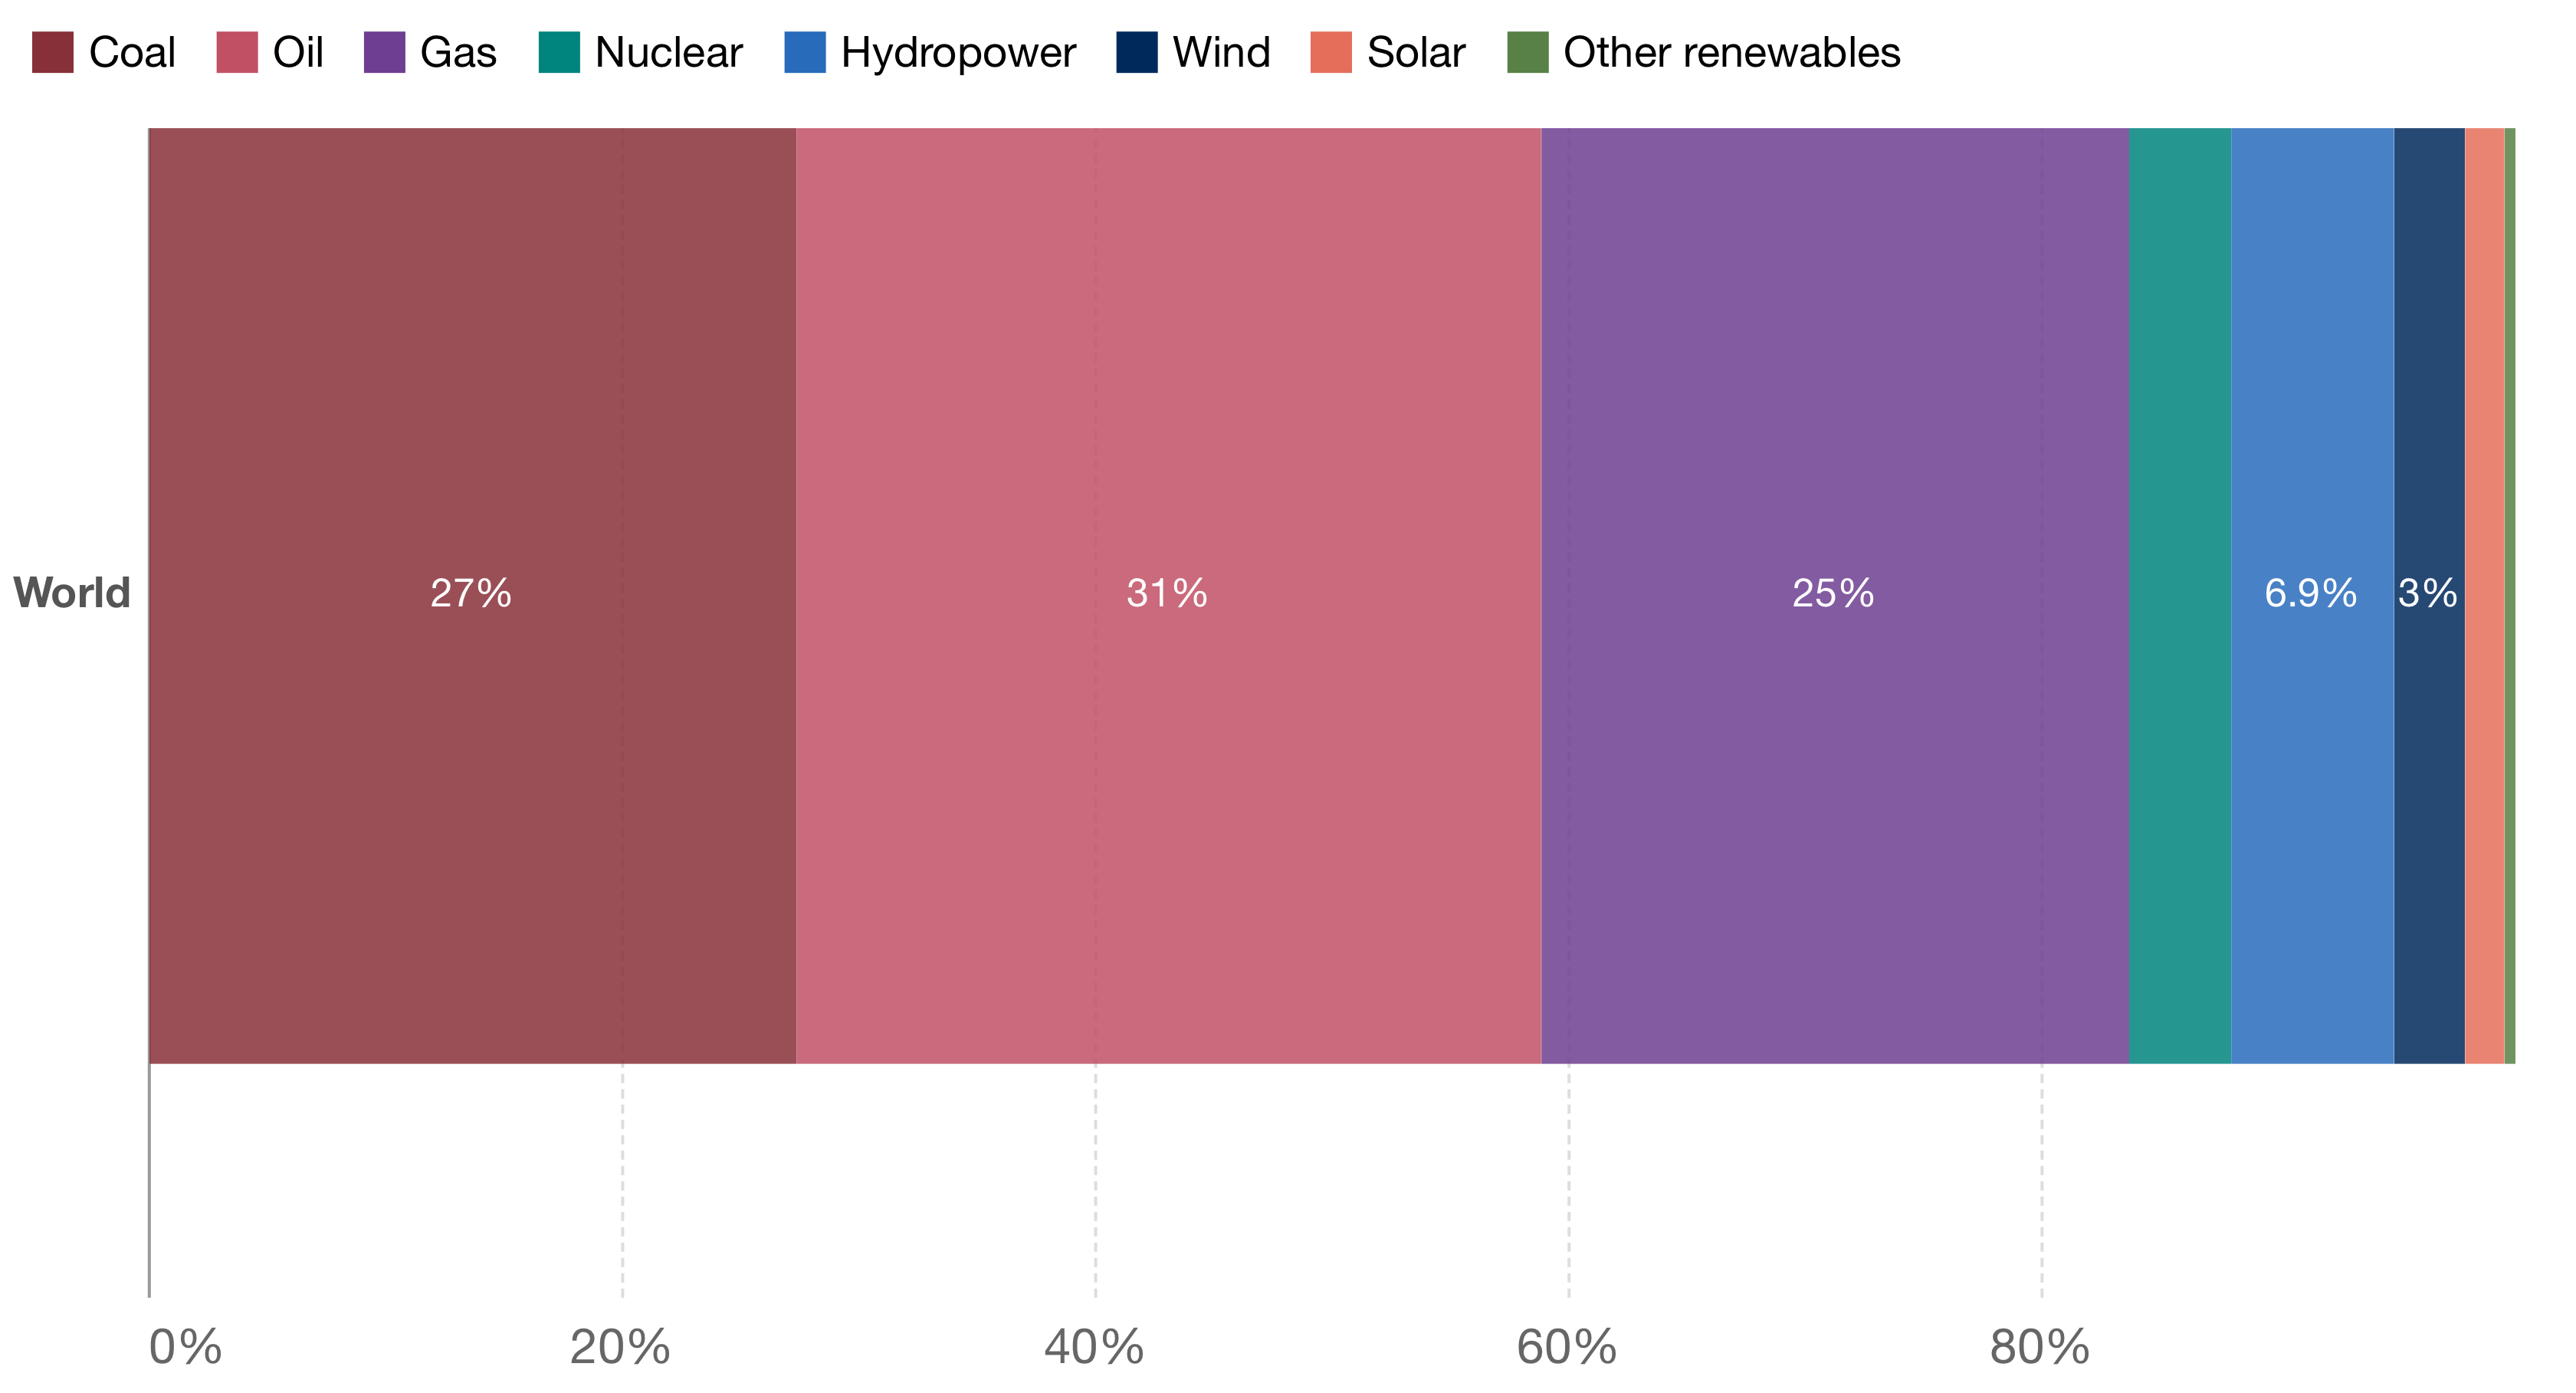
\includegraphics[width=\linewidth]{images/primary-energy-source-bar.png}
    \caption{Energy consumption by source, for China, Mexico, France, and the World \citep{ritchieWhichSourcesDoes2021}.}
    \label{fig.energy consumption}
\end{figure}

\subsubsection{Fossil fuels}
The second class of energy source is the fossil fuels, such as coal, oil and natural gas. These fuels are formed from the remains of plants and animals over millions of year. Once extracted, these fuels can be burnt to generate electricity, power motors, or, in the case of oil, can be used as raw material for a wide variety of products, including plastic, chemicals and pharmaceuticals. These energy sources, thanks to their high power density, powered the industrial revolution, and are the foundation of our civilization in the 21st century. Fossil fuels do not suffer from the same shortcomings as renewable energy source --- they are not intermittent, and can easily be turned on and off to follow the demand. Their land usage can be relatively small. For example, gas power plants uses $1\text{m}^2$ per MWh, about ten times less land than renewable energy sources. 

They however have many downsides. First and foremost, being non-renewable, there is only a limited amount of fossil fuels on Earth, which will eventually run out. Even if all disadvantages of fossil fuels are somehow avoided, humanity will have to move away from an economy based on fossil fuels because of their limited amount. Given the known reserves and the worldwide consumption of fossil fuels in 2020, humanity will exhaust supplies of coal in 139 years, of oil in 54 years, and of gas in 49 years \citep{bpBPStatisticalReview2020}. Another disadvantage is that the consumption of fossil fuels is one of the main source of greenhouse gases, which contribute to global warming and climate change \citep{allanIPCC2021Summary}. Fossil fuels are not globally well distributed, which is the source of multiple inequalities and to numerous geopolitical instabilities around the world. Finally, the fuel often has to be transported from its extraction location to the power plant, which requires large infrastructures, and consumes energy.

\subsubsection{Nuclear energy}
Another class of energy source is nuclear energy. Today, nuclear power plants produce electricity by leveraging the nuclear fission of Uranium. Fission power plants operation do not generate any greenhouse gases, are not intermittent, and are routinely used to generate electricity for base-load consumption. The large energy density of Uranium means that nuclear power plant have the best land to kWh ratio, with $0.3\text{m}^2$ per kWh. Tens of nuclear reactors can be enough to power a country.

The Uranium is however not well distributed globally, and is mainly being mined in Kazakhstan, Canada, Australia and Niger. Again, as for fossil fuel, this uneven distribution of resources is the source of geopolitical instabilities. Uranium is not renewable, and the world will eventually run out of fuel. According to the World Nuclear Association \citep{worldnuclearassociationUraniumSuppliesSupply2022}, the world's current annual consumption of uranium is around 61,000 tons per year. If this rate of consumption were to continue, the known land resources of uranium would last for around 90 years. However, this is a very rough estimate and does not take into account a number of factors that could affect the availability and use of uranium, such as the development of breeder reactors, changes in demand for electricity, or the exploitation of sea-water uranium ($4.6$ billion tons of uranium) \citep{dunganUraniumSeawaterInfinite2017}. Another downside to nuclear fission is that the reaction generates long-lived nuclear wastes dangerous for living organisms. In addition, the risk of loss of control of the power plant, such as during the infamous accidents of Chernobyl in 1986 and Fukushima in 2011, can lead to catastrophic releases of nuclear material in the atmosphere. New power plant designs, with smaller amount of fissing materials in their core, and additional safety measures, can however make their use safer.  Despite these disadvantages, nuclear fission is today the only energy source that can generate the amount of energy our civilization consumes without releasing greenhouse gases and without the inherent variability of renewable energies.

There are thus three pathways for future energy production: either massive structures are built across the globe to generate enough renewable energy, or massive funding is invested in developing and constructing new generations of fission nuclear power plant. The final pathway is exploiting a new source of energy that has not been discussed in the above discussion: \emph{nuclear fusion}. The advantages of nuclear fusion as a source of energy are numerous: the reaction does not generate any greenhouse gases, and, as for fission power and fossil fuels, is not intermittent. The considered fuel is Deuterium and Tritium, two isotopes of Hydrogen. Deuterium can be found in sea water, at a concentration of 155 part per millions (ppm), while Tritium is found in extremely small quantities on Earth, but can be produced by exposing lithium to a neutron flux,
\begin{equation}
    \ce{^{6}_{3}Li + ^{1}_{0}n -> ^{4}_{2}He + ^{3}_{1}T}.
\end{equation}
Lithium 6 is found in natural lithium, at a concentration of $7.5\%$. Though lithium is not equally distributed on Earth, extraction from seawater \citep{ZHAO2019113389} could be a future solution to this issue. Nuclear fusion does not face the same problematic as nuclear fission regarding nuclear wastes, as the reaction does not produce any radioactive materials. The reactor itself, exposed to neutron fluxes, is activated, and its materials have to be securely stored once decommissioned. These nuclear wastes are however short-lived in comparison to the nuclear wastes generated by nuclear fission. Finally, nuclear fusion reactors are intrinsically safe, as the reaction is not a chain reaction, and thus cannot undergo a core meltdown as nuclear fission reactors. Nuclear fusion comes also with a few disadvantages. As of today, the proposed reactor prototypes are large and expensive to build, and require a large upfront investment. Reaching the conditions for fusion is extremely difficult, and there are no reactor concept that has yet proven a net production of electricity. The National Ignition Facility (NIF) recently achieved a net power gain \citep{NationalIgnitionFacility} on the fusion fuel, but is still far from a net energy gain when taking into account all the power plant energy consumption.

\section{Nuclear fusion as a source of energy}
Nuclear fusion is the process of forming a nucleus from two, lighter nuclei. This is the process that powers all stars in the universe, and that will power future fusion nuclear reactors. Nuclear \emph{fusion} is the opposite of nuclear \emph{fission}, where two nuclei are formed by breaking one, heavier nucleus, which is commonly used to power today's nuclear fission power plants.

Atomic nuclei are composed of neutron and protons, and are kept bound together by the strong interaction. The binding energy of the nucleon, defined as the minimum energy required to separate a nucleus as a collection of its nucleon, measures then how tightly bound a nucleus is. The binding energy per nucleon, shown on Figure \ref{fig. binding energy}, is low for hydrogen, grows with atomic number until reaching a maximum for the iron, and then decreases with increasing atomic number. In general, fusing two nuclei lighter than iron will then release energy, and so does fissing one nucleus heavier than iron.

\begin{figure}
    \centering
    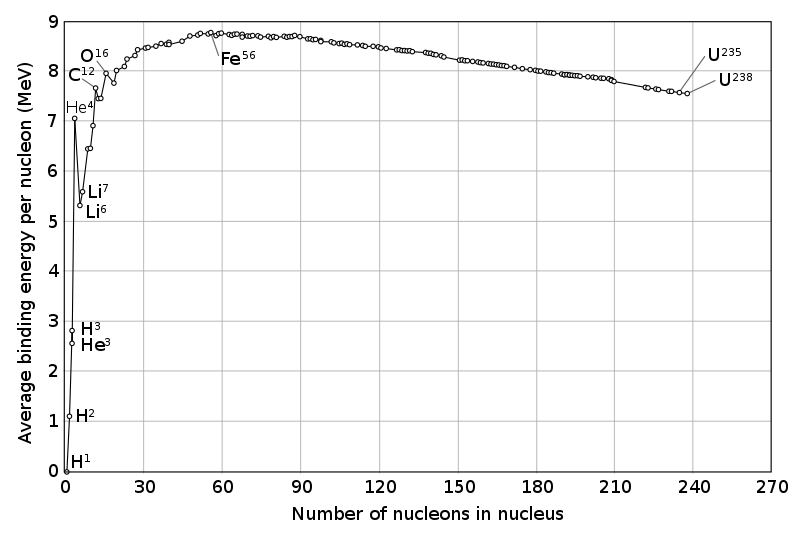
\includegraphics[width=.75\linewidth]{images/Introduction/BindingEnergy.png}
    \caption{Binding energy per nucleon. Credits: \url{https://tinyurl.com/4bmsrm3s}}
    \label{fig. binding energy}
\end{figure}

Of particular interest for commercial fusion power plants is the fusion of deuterium $\ce{H2}$ with tritium $\ce{H3}$, which generates a nucleus of helium $\ce{He4}$ with $3.5$MeV of kinetic energy, and a neutron with $14.1$MeV of kinetic energy (see Figure \ref{fig. dt fusion}). Among potential fusion reactions, this is the most promising, because the reaction cross-section is the highest. Nevertheless, deuterium-tritium fusion reactions require a temperature of at least $10$keV, \textit{i.e.} about 100 millions degrees. At these temperature, the fuel is a plasma, where electrons are stripped away from their nuclei. A plasma can be understood as a collection of electrons and ions, interacting with one another, and with external electromagnetic fields.
\begin{figure}
    \centering
    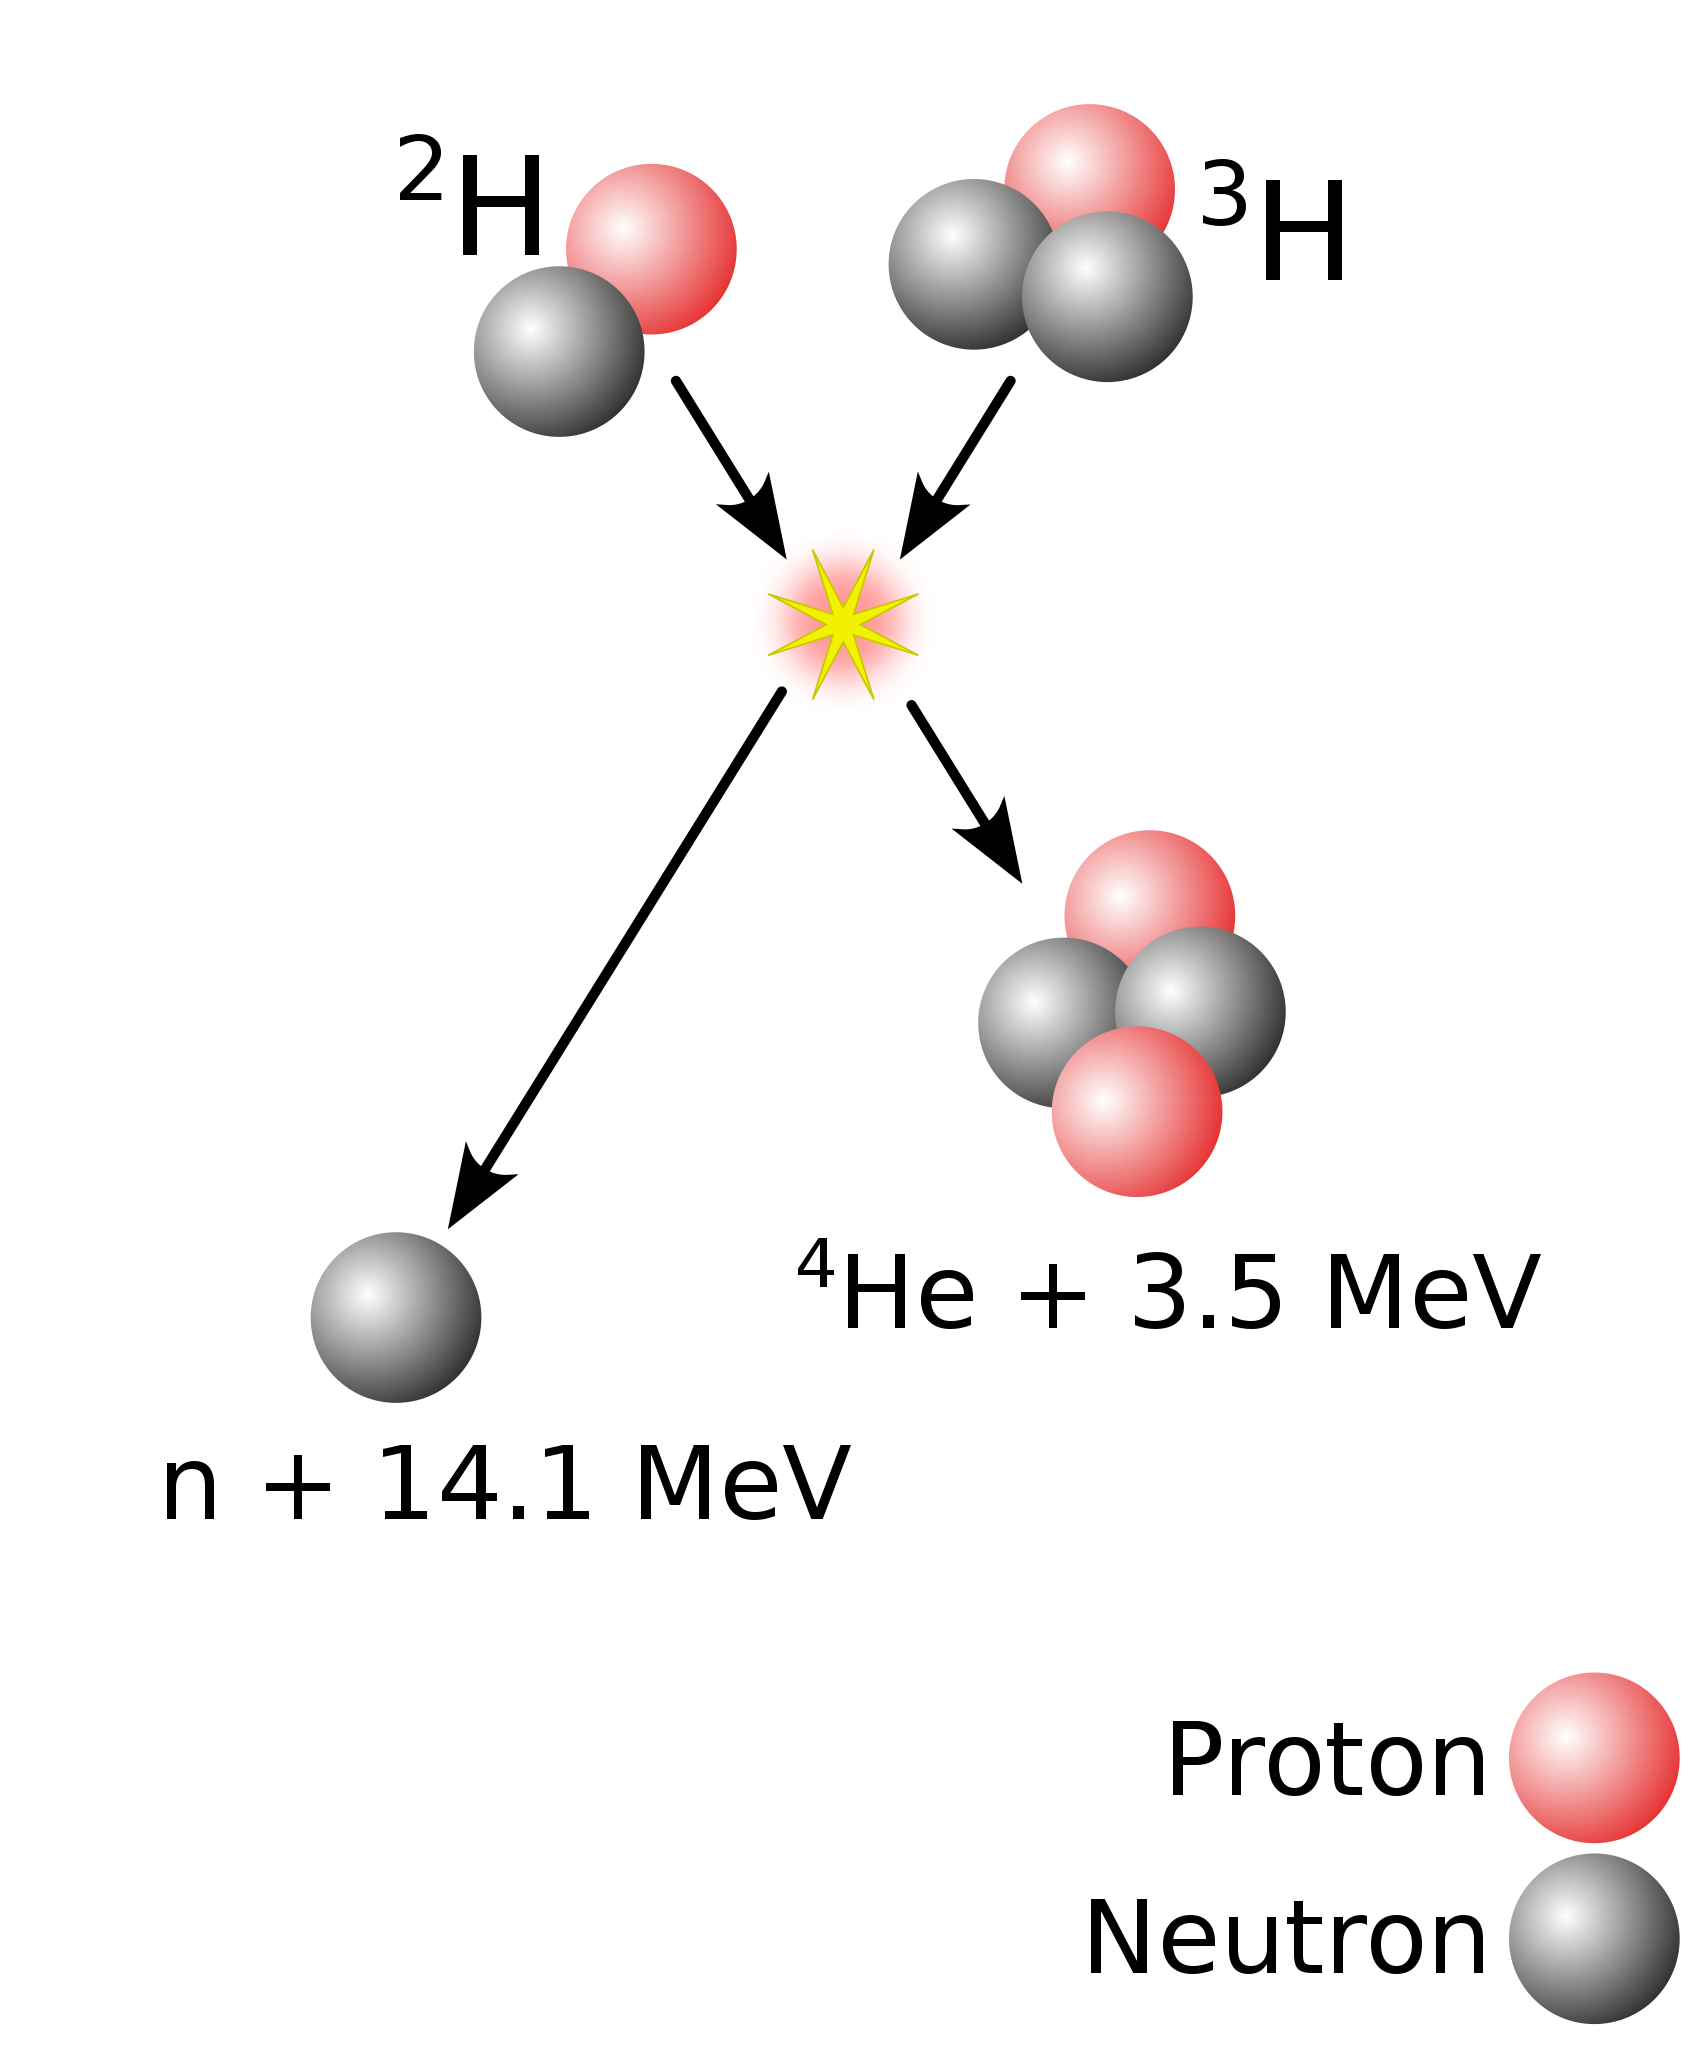
\includegraphics[width=.5\linewidth]{images/Introduction/DTFusion.png}
    \caption{Sketch of a Deuterium-Tritium fusion reaction. Credits: \url{https://tinyurl.com/3kyvakb4}}
    \label{fig. dt fusion}
\end{figure}

The challenge is then to confine the fuel for a sufficiently long time such that enough reactions have the time to occur. More specifically, we define the $Q$-factor as the ratio of power generated by the fusion reactions over the input power required to power the reactor, $Q=P_{fus}/P_{in}=1$. To get energy break-even, \textit{i.e.} to get as much fusion power as input power, $Q=1$, one can derive the so-called Lawson criterion \citep{lawsonCriteriaPowerProducing1957}, which gives a criterion on the fusion triple product,
\begin{equation}
    nT\tau_E > 1.5\cdot 10^{21}\text{keV s m}^{-3}, \label{eq. lawson criterion}
\end{equation} 
where $n$ is the plasma density, $T$ is its temperature, and $\tau_E$ is the energy confinement time. In addition, the plasma temperature cannot be too low nor too large, otherwise the fusion cross-section would be too small and Bremsstrahlung losses would fully compensate the generated fusion power. From the Lawson criterion (\ref{eq. lawson criterion}), one can identify two paths toward a nuclear fusion power plant: (i) inertial fusion, where one maximizes the density for a very short amount of time, but does not confine the plasma, or (ii) magnetic confinement, where one keeps comparatively lower densities, but increases as much as possible the energy confinement time by confining the plasma using carefully designed magnetic fields. This thesis will focus on one particular design of magnetic confinement reactor called the stellarator, which we explain in the section \ref{sec.stellarator concept}.


\section{Magnetic fusion reactor concepts} 
We discuss here how a magnetic field can be used to confine a plasma. The Virial theorem \citep{Freidberg2014} states that a plasma cannot generate a magnetic field to confine itself; an external magnetic field needs to be provided. In general, electromagnets are used to generate the external magnetic field, though configurations with permanent magnets have been proposed as well \citep{qianSimplerOptimizedStellarators2022,zhuPM4StellPrototypePermanent2022}. To confine a plasma, one must design a magnetic field that does not cancel anywhere in space --- otherwise the plasma would escape through this "hole" in the magnetic field. At first, one may think that the plasma can be shaped as a sphere. The hairy ball theorem \citep{Renteln2013-uu} however shows that there are no continuous tangent field that does not vanish anywhere on a sphere in 3-dimensional space. In fact, the only shape in 3D space with non-vanishing continuous vector field is a torus (or a Klein bottle, but these are non-realistic shapes for a reactor). A magnetic fusion reactor must thus shape the plasma into a shape homeomorphic to a torus (see Figure \ref{fig.torus}).  In what follows, we will define the toroidal direction as the long way around the torus, and the poloidal direction as the short way around it. We discuss now shortly the motion of a single particle in a toroidal magnetic field.

\begin{figure}
    \centering
    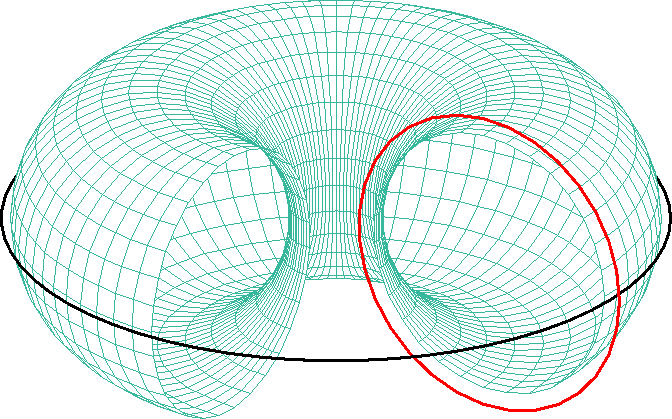
\includegraphics[width=.75\linewidth]{images/torus.png}
    \caption{Sketch of a torus. The red line follows the poloidal direction, while the black line follows the toroidal direction.}
    \label{fig.torus}
\end{figure}

\subsection{Single particle confinement}\label{sec.single particle confinement}
In a magnetic field, single particles move freely along the magnetic field lines, and move in circles around the magnetic field line in the perpendicular plane, thereby describing a gyromotion, with radius $\rho$ and frequency $\omega$, given by
\begin{align}
    \rho &= \frac{v_\perp}{\omega}\label{eq.gyroradius}\\
    \omega &= \frac{|q|B}{m},
\end{align}
where $v_\perp$ is the velocity of the particle perpendicular to the magnetic field line, $q$ is the charge of the particle, $B$ is the magnetic field strength, and $m$ is the particle's mass. The dynamics of single particles in a magnetic field can be greatly simplified if the magnetic field varies on scales larger than the gyroradius, $\rho|\nabla B|\ll B$, and that the magnetic field variations in time are much slower than a gyroperiod, $1/\omega \partial B/\partial t \ll B$. The equations of motion can then be averaged over a gyroperiod, and the motion of the particle is described by the trajectory of its guiding center (see Figure \ref{fig.gyromotion}).

\begin{figure}
    \centering
    \begin{tikzpicture}
        \node (fig) at (0,0) {
            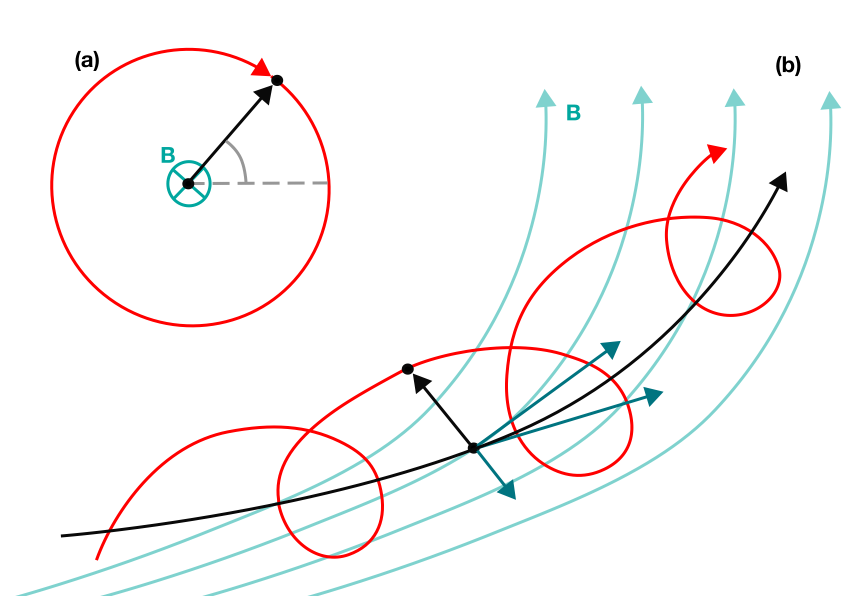
\includegraphics[width=\linewidth]{images/gyromotion.png}
        };
        \node (t1) at (-3.5,3.25) {$\rho\mathbf{s}$};
        \node (t2) at (-4,1.35) {$\mathbf{r}$};
        \node (t3) at (-2.25,4.15) {$\mathbf{x}$};
        \node (t4) at (-2.75,2.5) {$\gamma$};
        \node (t5) at (-0.25,-0.9) {$\mathbf{x}$};
        \node (t6) at (1,-2.25) {$\mathbf{r}$};
        \node[fill=white] (t7) at (2,-3.95) {$\mathbf{V}_E+\mathbf{V}_{\nabla B}+\mathbf{V}_\kappa$};
        \node (t8) at (4.5,-1.5) {$\mathbf{u}$};
        \node (t9) at (3.5,-0.5) {$u_\parallel\hat{\mathbf{b}}$};
    \end{tikzpicture}
    \caption{Sketch of a charged particle trajectory in a magnetic field. Figure (a) shows the trajectory in the plane perpendicular to the magnetic field, while Figure (b) shows the 3-dimensional trajectory. The light blue lines are the magnetic field lines, the red curve is the particle's trajectory, the black line is the particle's guiding center trajectory, and the dark blue arrows are the particle's velocity vectors.}
    \label{fig.gyromotion}
\end{figure}

We write the position of the particle as
\begin{equation}
    \mathbf{x} = \mathbf{r} + \rho\mathbf{s},\label{eq.single particle position}
\end{equation}
where $\mathbf{r}$ is the position of the gyrocenter, and $\mathbf{s}$ is a unit vector that rotates with the gyrophase $\gamma$. We require the gyroaverage of the second term on the right-hand side of Eq.(\ref{eq.single particle position}) to be zero, \textit{i.e.}
\begin{equation}
    \langle \rho\mathbf{s}\rangle_\gamma = \frac{1}{2\pi}\int_0^{2\pi} \rho\mathbf{s}d\gamma = 0,
\end{equation}
meaning that the vector $\mathbf{r}$ is the gyroaveraged position $\langle\mathbf{x}\rangle_\gamma = \langle\mathbf{r}\rangle_\gamma = \mathbf{r}$, which we call the guiding center. The particle velocity is then
\begin{equation}
    \mathbf{v} = \mathbf{u} + \frac{d\rho\mathbf{s}}{dt},
\end{equation}
with $\mathbf{v}=d\mathbf{x}/\mathbf{t}$ the particle velocity, and $\mathbf{u}=d\mathbf{r}/\mathbf{t}$ the guiding center velocity. Taking the equations of motion,
\begin{align}
    \frac{d\mathbf{v}}{dt} &= \frac{q}{m}(\mathbf{E}+\mathbf{v}\times\mathbf{B})\\
    \frac{d\mathbf{x}}{dt} &= \mathbf{v},
\end{align}
with $\mathbf{E}$ the electric field, one can show that the guiding center velocity in a electric and magnetic field at equilibrium (\textit{i.e.} time independent) can be written as a combination of three different drifts \citep{freidberg_2007},
\begin{equation}
    \mathbf{u} = \mathbf{V}_E + \mathbf{V}_{\nabla B} + \mathbf{V}_\kappa + u_\parallel \hat{\mathbf{b}},
\end{equation}
with $u_\parallel$ the velocity parallel to the magnetic field, $\hat{\mathbf{b}}=\mathbf{B}/B$, and
\begin{align}
    \text{The $\mathbf{E}\times\mathbf{B}$ drift}\qquad &\mathbf{V}_E = \frac{\mathbf{E}\times\mathbf{B}}{B^2}\\
    \text{The $\nabla B$ drift}\qquad &\mathbf{V}_{\nabla B} = \pm \frac{u_\perp^2}{2\omega}\frac{\mathbf{B}\times\nabla B}{B^2}\\
    \text{The curvature drift}\qquad &\mathbf{V}_\kappa = \pm \frac{v_\parallel}{\omega}\frac{\mathbf{R}_c\times\mathbf{B}}{R_c^2 B},
\end{align}
where the positive sign is taken for ions, the negative sign for electrons, $u_\perp$ is the guiding center velocity perpendicular to the magnetic field, and $\mathbf{R}_c$ is the curvature vector. Because of these drifts, the guiding center trajectory does not necessary follow a magnetic field line (see Figure \ref{fig.gyromotion} (b)).

Let's assume that we construct a magnetic fusion reactor with a purely toroidal magnetic field, $\mathbf{B}= B\mathbf{e}_\phi$, where $\mathbf{e}_\phi$ is a unit vector in the toroidal direction. To generate such a field, toroidal coils with a coil current $I_c$ have to be used. Leveraging Ampere's law, we get $B \sim I_c / 2\pi R$, \textit{i.e.} the magnetic field is stronger close the torus hole, and smaller on the outer side of the machine, thereby defining a "high-field side" and a "low-field side" to the machine. In such magnetic field, a single particle will experience both a $\nabla B$ drift and a curvature drift in the same vertical direction. Because both drifts direction depends on the sign of the particle electric charge, electrons will drift in the opposite direction as the ions, and a charge separation will appear. A vertical electric field will emerge, which, according to the $\mathbf{E}\times\mathbf{B}$ drift, will push the particles outside the torus, thereby losing confinement. A purely toroidal magnetic field is thus not sufficient for confining a plasma.

\begin{figure}
    \centering
    \begin{tikzpicture}
        \node (fig) at (0,0) {
            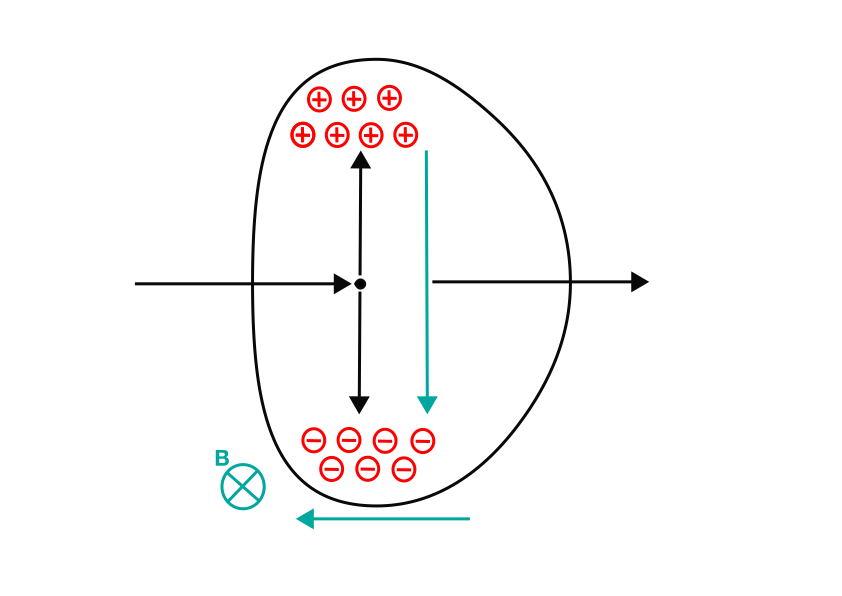
\includegraphics[width=\linewidth]{images/ToroidalField.png}
        };
        \node (t1) at (-2,0.55) {$R_c$};
        \node[fill=white] (t2) at (-1.5,1.5) {$\mathbf{V}_\kappa+\mathbf{V}_{\nabla B}$};
        \node[fill=white] (t3) at (-1.5,-1) {$\mathbf{V}_\kappa+\mathbf{V}_{\nabla B}$};
        \node (t4) at (-1.25,-4.25) {\color{Leman}$\nabla B$};
        \node (t5) at (0.5,-1.5) {\color{Leman}$\mathbf{E}$};
        \node (t6) at (3.5,0.75) {$\mathbf{V}_E$};
    \end{tikzpicture}
    \caption{Sketch of the guiding center drifts in a purely toroidal magnetic field (zero rotational transform).}
\end{figure}

Adding a poloidal component to the magnetic field solves this problem --- due to their motion parallel to the magnetic field lines, particles will move from the upper portion of the torus to the lower one, and vice versa, which prevents the charge separation to occur, stops the electric field to emerge, and ultimately provides confinement within the torus to the particles. A magnetic field with a poloidal component wraps around the torus both in the poloidal and toroidal direction. This magnetic field line twist is described mathematically by the \emph{rotational transform} $\iotabar$, which counts how many poloidal turns a magnetic field line does per toroidal turn. 

\subsection{Sources of rotational transform} 
There are three ways to twist magnetic field lines. The discussion relies on assuming that magnetic field lines lay on nested toroidal surfaces, with the magnetic axis the innermost (degenerate) surface. The magnetic axis is a line, described by $\mathbf{r}_0(l)$, with $l$ the arc length. We can define the so-called Frenet-Serret coordinate system $(\hat{\mathbf{e}}_1,\hat{\mathbf{e}}_2,\hat{\mathbf{e}}_3)$, with 
\begin{align}
    \text{The unit tangent vector}\qquad &\hat{\mathbf{e}}_1=\frac{d\mathbf{r}_0}{dl} = \hat{\mathbf{b}}\\
    \text{The unit curvature vector}\qquad &\hat{\mathbf{e}}_2=\frac{1}{\kappa}\frac{d\hat{\mathbf{e}}_1}{dl}\\
    \text{The unit torsion vector}\qquad &\frac{d\hat{\mathbf{e}}_3}{dl}= -\tau \hat{\mathbf{e}}_2,
\end{align} 
with $\kappa$ the curvature and $\tau$ the torsion. It can be shown \citep{mercierEquilibriumStabilityToroidal1964,helanderTheoryPlasmaConfinement2014} that the rotational transform on the magnetic axis is
\begin{equation}
    \iotabar_{axis} = \frac{1}{2\pi}\int\left[\frac{\mu_0 J}{2B_0}-(\cosh\eta-1)d'-\tau\right]\frac{dl}{\cosh\eta} - N,
\end{equation}
with $\mu_0$ the vacuum permeability, $J$ and $B_0$ the parallel current density and the magnetic field magnitude on the axis respectively, $\eta$ is related to the ellipticity of magnetic surfaces close to the magnetic axis, $d$ is the angle between the ellipse's minor radius and the unit curvature vector $\hat{\mathbf{e}}_2$, the prime denotes a derivative with respect to $l$, and $N$ counts the number of rotations of the magnetic axis curvature vector around the magnetic axis for one toroidal transit (see Figure \ref{fig.near axis expansion}). 

\begin{figure}
    \centering
    \begin{tikzpicture}
        \node (fig) at (0,0) {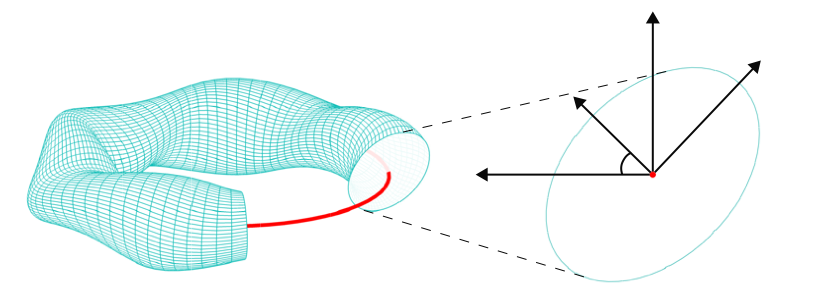
\includegraphics[width=\linewidth]{images/ellipse.png}};
        \node (e2) at (2,0) {$\mathbf{\hat{e}}_2$};
        \node (e3) at (4.5,2.75) {$\mathbf{\hat{e}}_3$};
        \node (x) at (3,0.6) {$\mathbf{x}$};
        \node (y) at (6.5,1.5) {$\mathbf{y}$};
        \node (d) at (3.5,-0.1) {$d$};
    \end{tikzpicture}
    \caption{Illustration of an elliptical magnetic surface close to the magnetic axis. In red: the magnetic axis; In blue: the magnetic surface. The $\mathbf{x}$ and $\mathbf{y}$ axes are in the direction of the ellipse minor and major radii respectively.}
    \label{fig.near axis expansion}
\end{figure}


The rotational transform can thus be generated by three mechanisms: (i) by driving a toroidal current $J>0$ in the plasma, or (ii) by shaping the magnetic surfaces as rotating ellipses close to the axis, with $\eta\neq 0$ and $d\neq 0\ \forall\phi$, or (iii) by having magnetic axis torsion, \textit{i.e.} $\tau\neq 0$. The two main classes of magnetic confinement devices, the tokamak and the stellarator, rely on different mechanisms to generate the rotational transform.

\subsection{The tokamak concept}
The tokamak, arguably the most advanced concept for a fusion reactor, uses an external transformer to drive a strong toroidal current in the plasma in order to generate the rotational transform (see Figure \ref{fig tokamak sketch}). One of its great advantage is that the configuration is axisymmetric --- \textit{i.e.} there are no dependencies on the toroidal position. This property implies good neo-classical confinement, and, from an engineering point of view, makes the tokamak a relatively simple reactor to build. Driving a strong toroidal current comes however with some disadvantages --- the operation of the machine is intrinsically pulsed, forbidding continuous operation and generating stress on the different components, ultimately reducing the lifetime of the machine, and driving up the cost of electricity. The current is also a source of free energy in the plasma, which can generate powerful instabilities that have to be controlled. Tokamaks therefore require extensive diagnostics and real time control for operation \citep{degraveMagneticControlTokamak2022}. We can summarize the tokamak concept as a device relatively simple to build, but complex to operate.

\begin{figure}
    \centering
    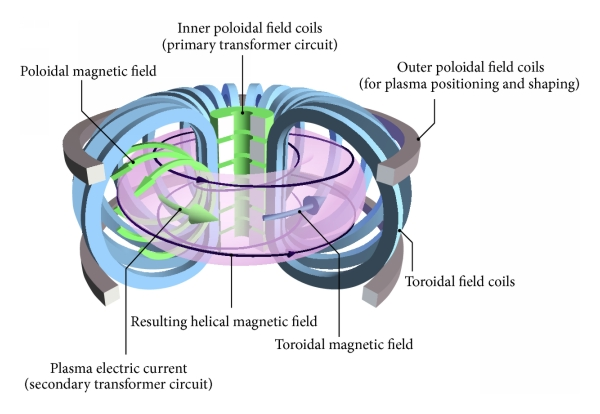
\includegraphics[width=\linewidth]{images/Introduction/TokamakSketch.jpg}
    \caption{Schematic of a tokamak. Credits: \url{https://tinyurl.com/bdfn3tc7}}
    \label{fig tokamak sketch}
\end{figure}

\subsection{The stellarator concept}\label{sec.stellarator concept}
The stellarator uses all three mechanisms to generate the rotational transform. In practice however, the generation of a toroidal current is often not considered, as it would imply the same disadvantages as the tokamak, \textit{i.e.} it would require the installation of a transformer, continuous operation would be impossible, and current-driven instabilities would need to be controlled. Instead, the stellarator relies on the ellipticity of the magnetic surfaces and their rotation, $\eta\neq0$ and $d = d(l)$, and on the magnetic axis torsion, $\tau\neq0$. This means that the magnetic field can be entirely generated by external coils, there is no need for a central transformer, and the machine can be operated continuously. There are no current-driven instabilities (unless the plasma generates its own current), meaning that disruptions (loss of control of the plasma) are less common in stellarators than in tokamaks.

The rotation of the elliptical magnetic surfaces and the magnetic axis torsion come however at the cost of losing axisymmetry: the configuration is now fully 3-dimensional (see Figure \ref{fig stellarator sketch}). The neo-classical transport is in general worse than in tokamaks, and extensive additional optimization is required to obtain good confinement properties. In addition, the 3-dimensionality of the coils and their necessary precise positioning is a formidable engineering challenge, and can increase the cost of the machine substantially. The National Compact Stellarator Experiment (NCSX), for example, was canceled on 22 May 2008 \citep{orbachFuturePrincetonPlasma2008}, due to "the budget increases, schedule delays and continuing uncertainties" of the NCSX experiment. The stellarator concept can then be summarized as a machine that is hard to build but easy to operate. 

\begin{figure}
    \centering
    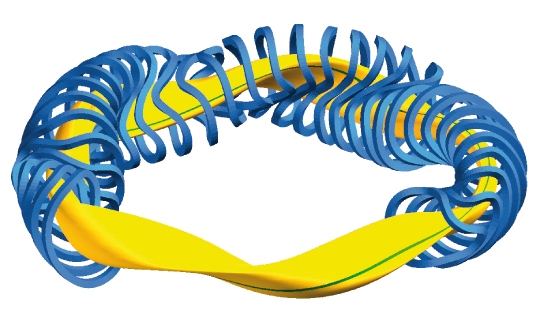
\includegraphics[width=\linewidth]{images/Introduction/StellaratorSketch.jpg}
    \caption{Schematic of a stellarator. Credits: \url{https://tinyurl.com/5ppm845w}}
    \label{fig stellarator sketch}
\end{figure}

Thanks to the 3D nature of stellarators, their configuration space is orders of magnitude greater than tokamaks. Stellarators can thus be optimized for different properties, for example quasi-symmetry \citep{Landreman2022}, quasi-isodynamicity \citep{goodmanConstructingPreciselyQuasiisodynamic2022a},  or low turbulent transport \citep{xanthopoulosControllingTurbulencePresent2014}. The Wendelstein-7X stellarator, for example, has been optimized for low neo-classical transport, which has been verified experimentally \citep{beidlerDemonstrationReducedNeoclassical2021}. Recent advances in stellarator optimization improved the confinement properties of stellarators beyond what can be achieved by a tokamak \citep{landremanOptimizationQuasisymmetricStellarators2022}. These optimizations are however often done in vacuum; pressure and currents interact with the equilibrium properties through complex non-linear equations. In particular, magnetic field equilibria can be perturbed by pressure induced currents, and the topology of field lines can be modified, potentially losing the confinement properties of the magnetic field. We discuss, in the next section, the possible magnetic field line topologies in toroidal magnetic fields.
%Quasi-isodynamics \citep{goodmanConstructingPreciselyQuasiisodynamic2022a} and quasi-symmetric \citep{Landreman2022} fields have been found


\section{Magnetic field line topologies}
We discuss here the phenomenology of magnetic equilibria, and what kind of field line topologies can exist in toroidal equilibrium magnetic fields. Magnetic equilibria are, in general, composed of nested magnetic surfaces, magnetic islands and magnetic field line chaos (see Figure \ref{fig. topology examples}) \citep{helanderTheoryPlasmaConfinement2014}. The innermost magnetic surface is degenerate and is a line --- this is the so-called magnetic axis. In principle, it is possible to generate magnetic equilibria with multiple magnetic axis. In this thesis however, we will focus uniquely on single magnetic axis configurations. Measurements via injection of an electron beam in a dilute gas in the Wendelstein-7X stellarator \citep{pedersenConfirmationTopologyWendelstein2016}, built in Greisfwald, Germany, gave experimental evidence of the existence of magnetic surfaces (Figure \ref{fig w7x magnetic surface}) and of the edge magnetic island chain (Figure \ref{fig w7x magnetic island}).

\begin{figure}%
	\centering
	\subfloat[Magnetic surface]{\label{fig w7x magnetic surface}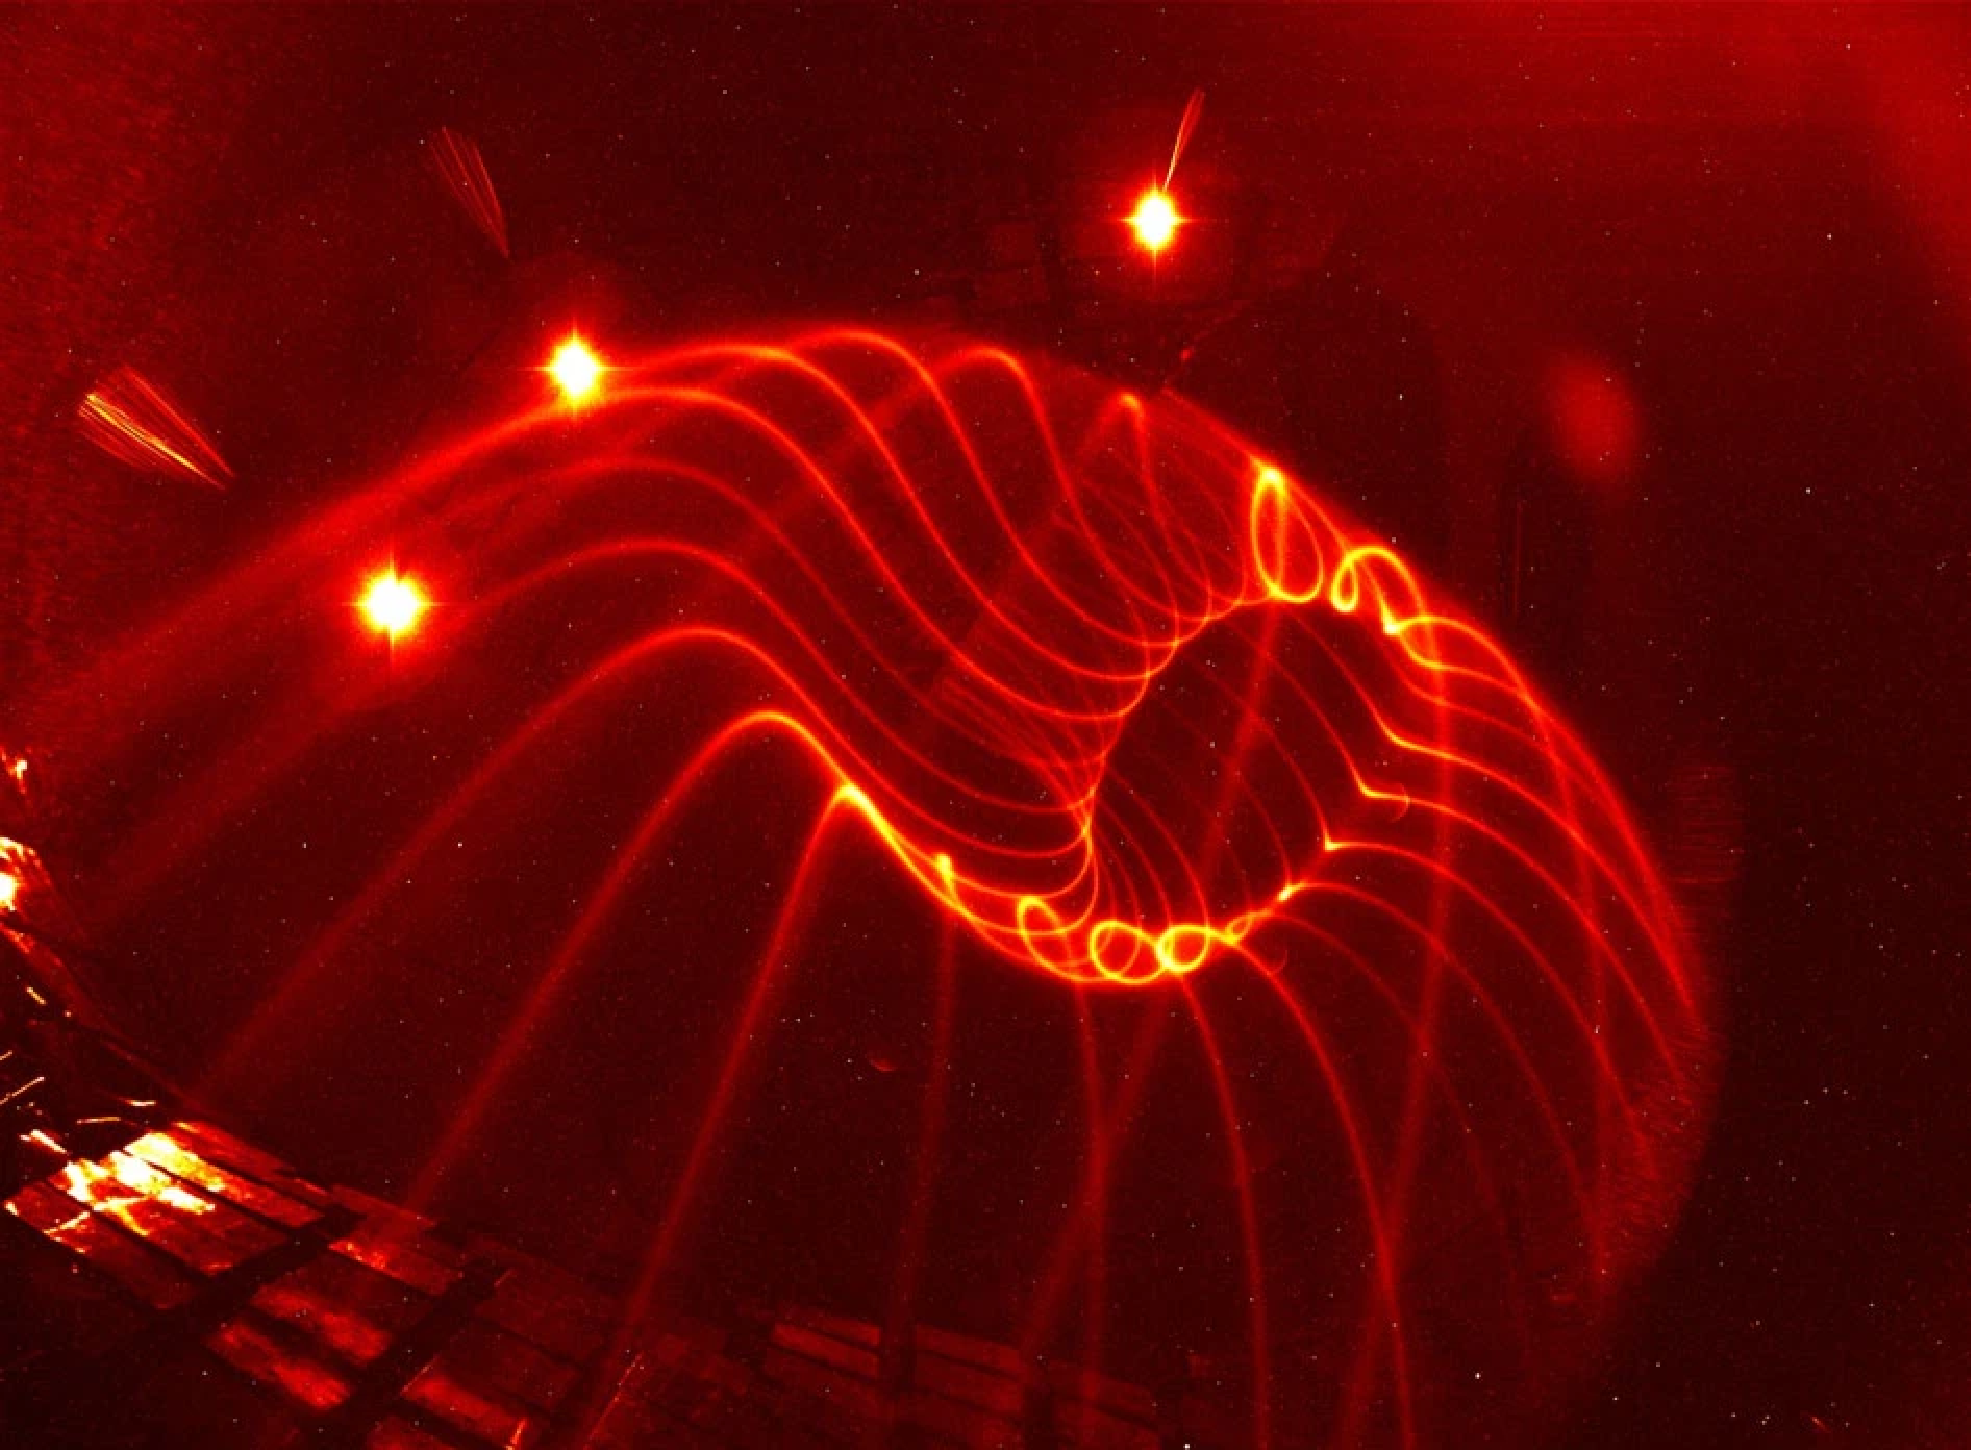
\includegraphics[height=4.8cm]{images/Pedersen2016_MagneticSurface_W7X.pdf}}%
	\qquad
	\subfloat[Magnetic islands]{\label{fig w7x magnetic island}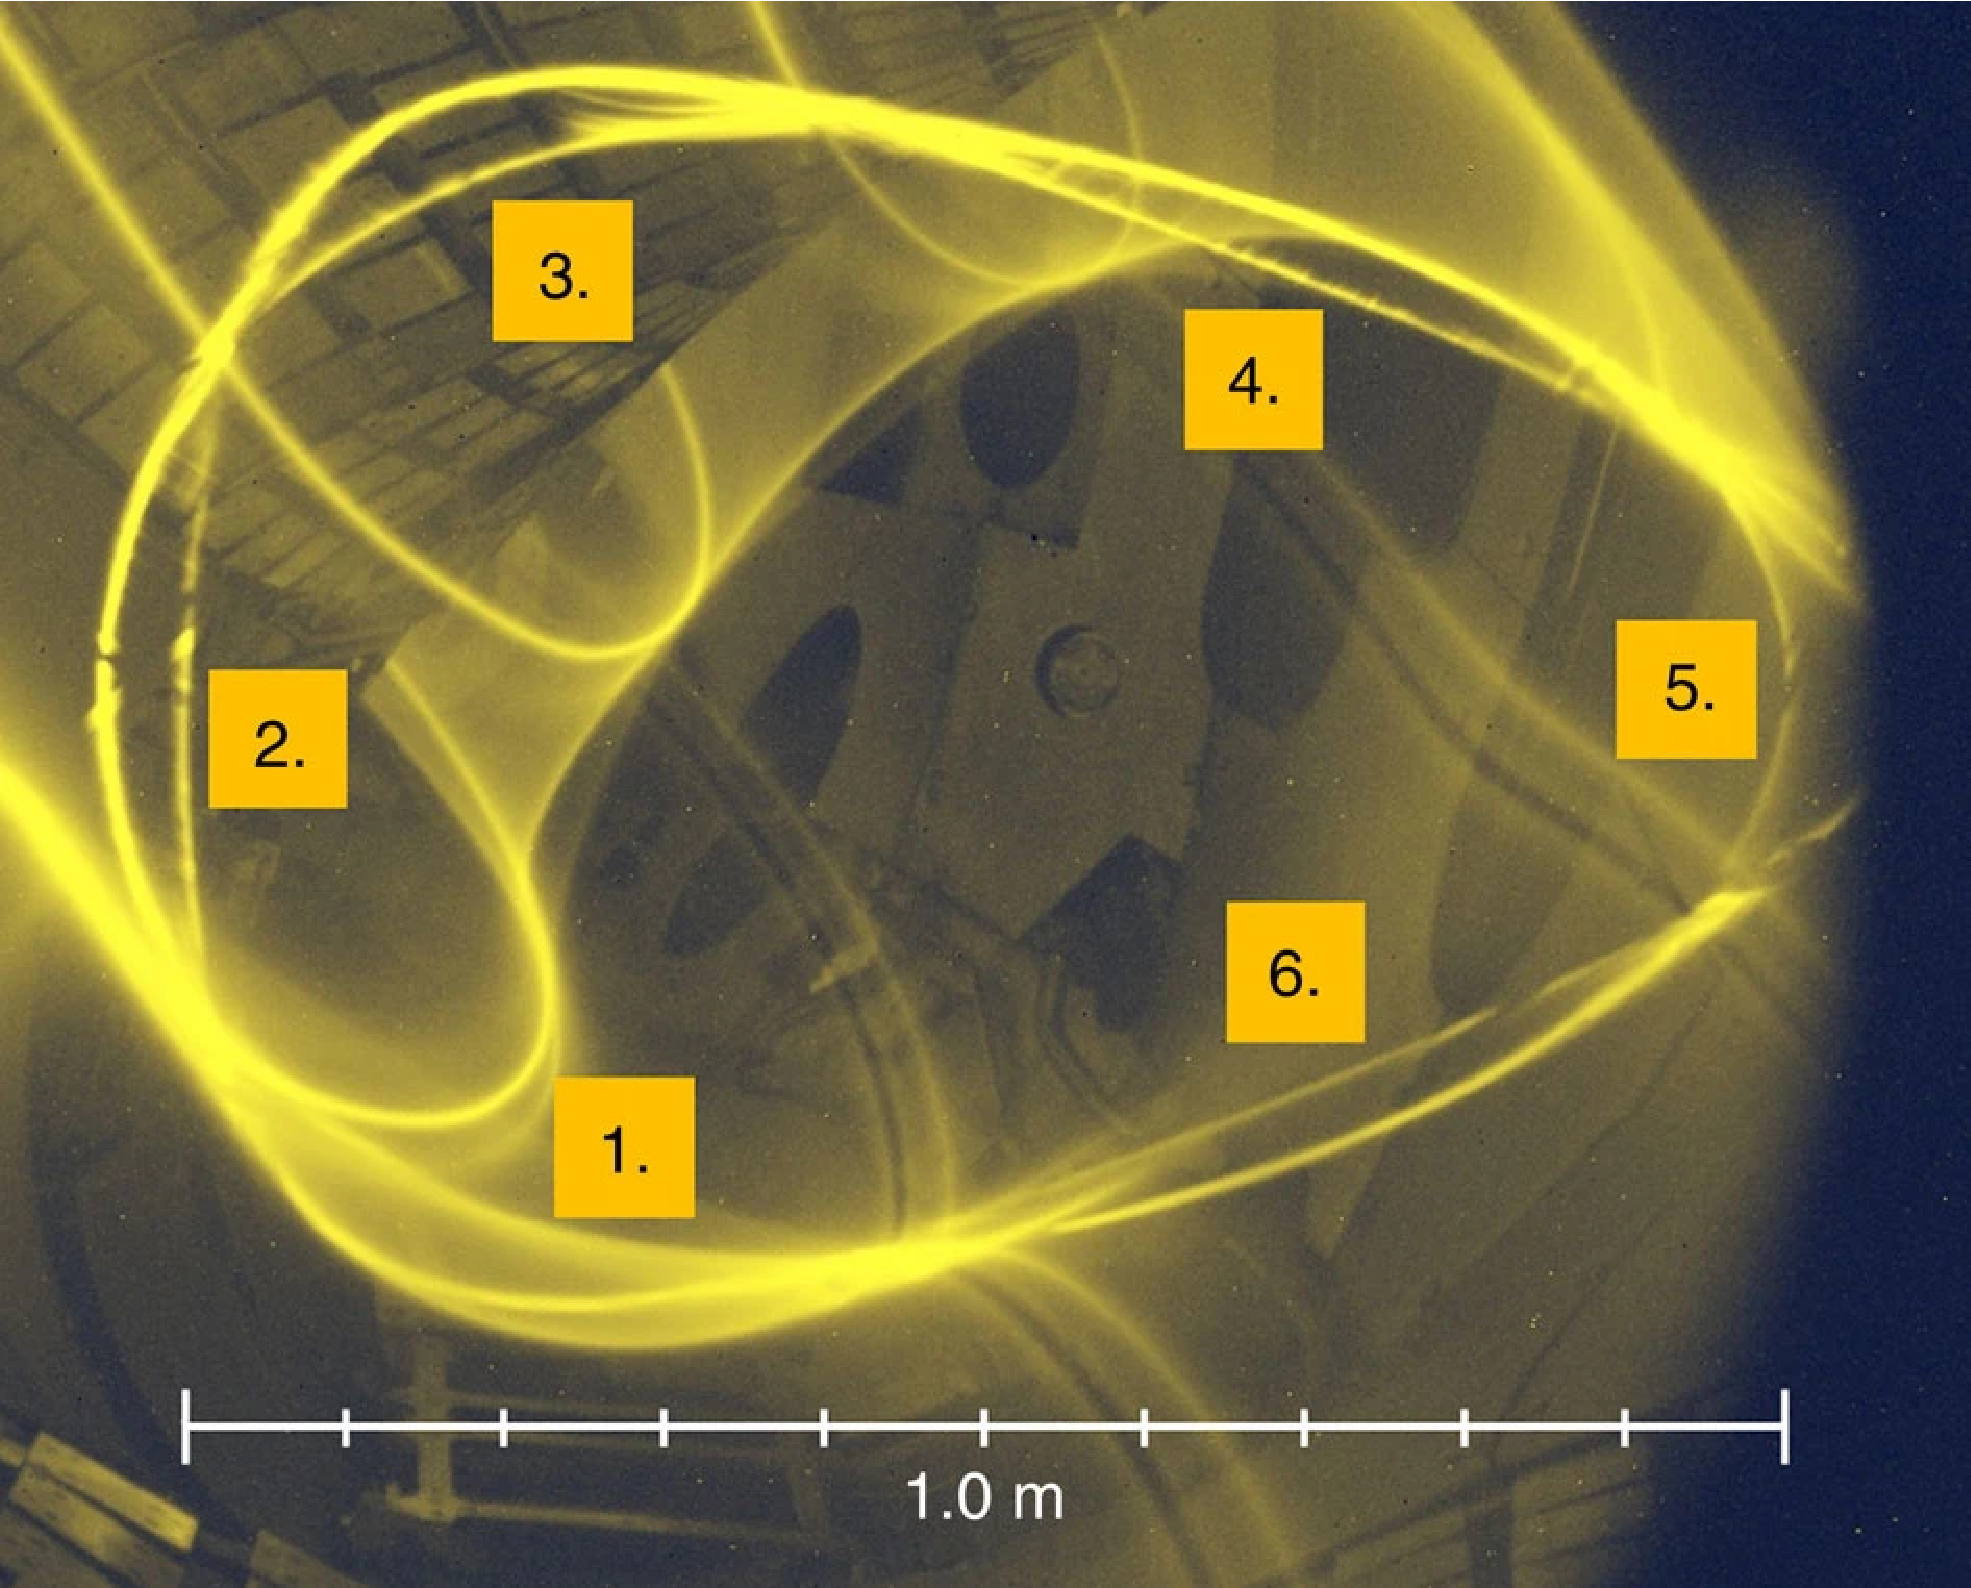
\includegraphics[height=4.8cm]{images/Pedersen2016_MagneticIsland_W7X.pdf}}
	\caption{Measurement of the field line topology in W7-X via injection of an electron beam in a dilute gas \citep{pedersenConfirmationTopologyWendelstein2016}.}
	\label{fig. w7x topology measurement}%
\end{figure}

Now, suppose that an equilibrium is given --- by that, we mean that the magnetic field $\mathbf{B}$ is known everywhere, \textit{i.e.} at any position $(r,\theta,\phi)$, where r is a radial coordinate, $\theta$ is a poloidal angle and $\phi$ is the usual cylindrical toroidal angle, and $\mathbf{B}$ is independent of time. To visually see the magnetic field line topologies, a Poincare section can be plotted. To do so, the field lines are followed by solving the differential equation
\begin{equation}
	\frac{d\theta}{d\phi} = \frac{\mathbf{B}\cdot\nabla\theta}{\mathbf{B}\cdot\nabla\phi},
\end{equation}
with initial condition $r(0)=r_0$, $\theta(0)=\theta_0$ where $(r_0,\theta_0)$ are the initial field line position at $\phi=0$. An example of a field line followed on a magnetic surface is shown on Figure \ref{fig. field line tracing}. The field line is followed for multiple toroidal transits, and its position $(r_k,\theta_k)$ is saved whenever $\phi=2k\pi$, with $k\in\mathbb{N}$. The Poincare section is then a collection of $(r_k,z_k)_{k=\{1,\ldots,N\}}$ positions, plotted on the $(R,Z)$ plane. An example of a Poincare section with different field line topologies is shown on Figure \ref{fig. topology examples}.

\begin{figure}
	\centering
	\subfloat[][Field line]{\label{fig. field line tracing}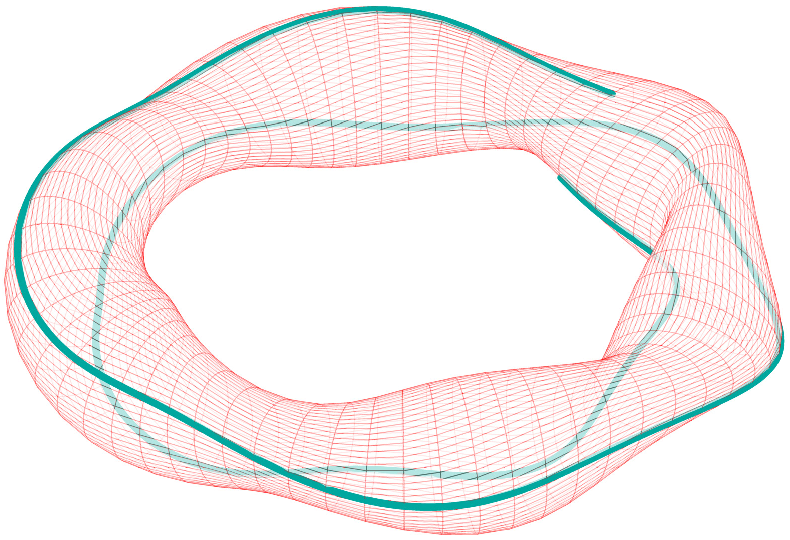
\includegraphics[height=4cm]{images/3d_field_line_tracing.pdf}}
	\hfill
	\subfloat[][Poincare section]{\label{fig. topology examples}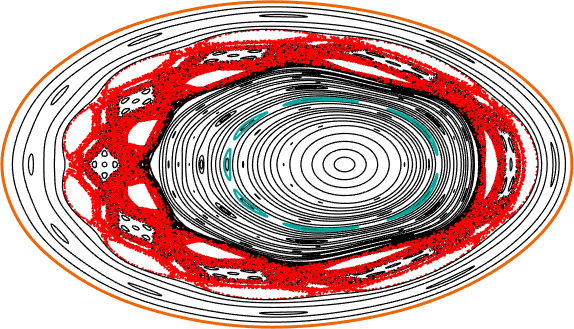
\includegraphics[height=4cm]{images/poincare_section_example.pdf}}
	\caption{Example of field line tracing and Poincare section in a rotating ellipse. Left: 3D mesh of a magnetic surface (red) and a traced field line over two periods (blue). Right: Poincare section of multiple field lines, with, in particular, a magnetic surface (orange), a magnetic island (blue) and a chaotic field line (red).}
	\label{fig poincare section}
\end{figure}

%Magnetic surfaces are toroidal surfaces on which the magnetic lays, \textit{i.e.} $\mathbf{B}\cdot\mathbf{n}=0$ with $\mathbf{n}$ a vector normal to the magnetic surface. In axisymmetric devices such as tokamaks, one can prove that nested magnetic surfaces exist everywhere, from the plasma edge to the magnetic axis, which is the innermost field line. Magnetic islands are formed when (i) the magnetic field is perturbed with a mode $\delta B_r \propto exp(i(m\theta-n\phi))$, with $(\theta,\phi)$ a poloidal and toroidal angle, and $m$, $n$ the poloidal and toroidal mode number, and (ii) the rotational transform is a rational number equal to $\iotabar=n/m$. Finally, magnetic field line chaos is formed when two or more island chains overlap --- this is the so-called Chirikov criterion \citep{Chirikov1979}. Further details about these magnetic field line topologies and their hamiltonian description can be found in the review paper by \citet{Meiss1992c} and references therein. 

%To accurately model and understand the physics in a stellarator, it is important to consider equilibria that allow magnetic islands and magnetic field line topologies. In the following chapter, we discuss important properties of the ideal \ac{MHD} model (section \ref{section ideal mhd}), the Taylor relaxation model (section \ref{section taylor state}) and of the \ac{MRxMHD} model (section \ref{section mrxmhd}).

Magnetic field line topologies are intrinsically connected to particle confinement. At zeroth order, particle and energy confinement is obtained on magnetic surfaces; magnetic islands and magnetic field line chaos, on the other hand, may increase radial transport, since particles following field lines with these topologies have orbits with finite radial excursion. This is however not the full story; structures in regions occupied by chaotic field lines can potentially support pressure gradient \citep{Hudson2008}, but in general the transport in these regions will be greater than in regions occupied by magnetic surfaces. We thus desire to design magnetic equilibria with a large volume occupied by magnetic surfaces. 


\section{Scope of this thesis}


It can be shown \citep{gradHydromagneticEquilibriaForcefree1958,shafranovPlasmaEquilibriumMagnetic1966,Freidberg2014} that all magnetic field lines lay on toroidally nested magnetic surfaces in axisymmetric configuration such as tokamaks, thereby avoiding the difficulties related to magnetic islands and magnetic field line chaos. Since stellarators are not axisymmetric, their magnetic equilibria may feature magnetic islands and magnetic field line chaos. Often, stellarator optimization are nevertheless performed while assuming the existence of magnetic surfaces. Once a configuration that extremizes the cost function is found, a few additional calculations and corrections are performed to remove potential islands \citep{Hanson1984a,Cary1986}. More recently, \citet{Landreman2021a} performed an optimization for quasi-symmetry at the same time as good magnetic surfaces in vacuum, clearly showing that multi-target stellarator optimization that includes good magnetic surfaces as a target are possible.

Carefully designed vacuum magnetic fields are however perturbed by plasma generated currents when the pressure is finite. For sufficiently large pressures, the vacuum magnetic field is perturbed enough for magnetic islands and magnetic chaos to emerge, which causes a degradation of the magnetic field confinement properties. This loss of magnetic surfaces consequently defines a so-called equilibrium pressure limit in the stellarator. This phenomenon is thought to be what limits the pressure in the stellarator \citep{helanderTheoryPlasmaConfinement2014}, and, ultimately, the machine performance. This is in contrast to tokamaks, where the pressure is limited by stability properties of the plasma; crossing the stability limit in a tokamak often leads to a loss of control of the plasma, \textit{i.e.} a disruption. The equilibrium pressure limit is however not well understood in stellarators, and there is no extensive analytical model to describe its dependance on the main machine's design parameters. 

This is where the work from this thesis fits in; the aim  is to  understand the equilibrium pressure limit in stellarators, and model its main parameter dependencies. In addition, we will show proof of principle calculations where the equilibrium pressure limit in a simplified stellarator geometry is optimized to a larger value than the un-optimized case. To reach these goals, we first describe different mathematical models for 3D MHD equilibria in chapter \ref{chap.3d magnetic equilibria}. In chapter \ref{ch3.SPEC} we describe \ac{SPEC}, a 3D MHD equilibrium code, and we implement new capabilities to compute free-boundary, finite pressure, finite current, 3-dimensional magnetohydrodynamic equilibria with magnetic islands and magnetic chaos. In chapter \ref{ch4.diagnostics} different numerical diagnostics to measure the confining properties of the magnetic equilibrium computed by SPEC are discussed. These diagnostics are leveraged in chapter \ref{ch5.equilibrium_beta_limit} to evaluate the equilibrium pressure limit in different stellarator configurations. Finally, we describe how \ac{SPEC} has been coupled with the SIMSOPT python framework for stellarator optimization \citep{Landreman2021b}, and explore the different degrees of freedom available for optimizing the equilibrium pressure limit in chapter \ref{ch6.optimization}.

% \begin{figure}
% \centering
% 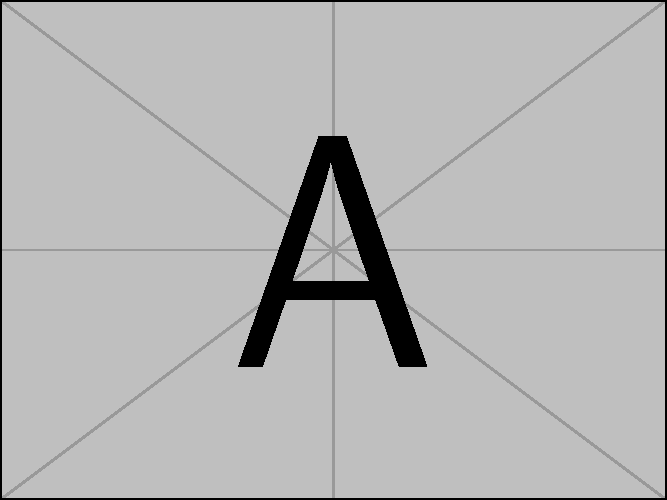
\includegraphics[width=\linewidth]{images/example-image-a.pdf}
% \caption{Example of a magnetic surface, a magnetic island chain and magnetic field line chaos.}
% \label{fig. topology examples}
% \end{figure}

%In the next sections, we will discuss different mathematical models that have been developed to describe 3D magnetic equilibria, \textit{i.e.} answering the question "\emph{Given a boundary, pressure and current profiles, what is the magnetic field in a plasma?}"

\end{document}


